\chapter{ALGORITMO FP-FLOCK}

En el algoritmo propuesto por \cite{VieiraT13}, en la primera parte del algoritmo se encuentra el total de discos con los 
objetos móviles que están juntos, se eliminan discos que no cumplan $\mu$, este proceso genera que se encuentren varios de
 los discos solapados, para ello, por último, se realiza una limpieza de los discos solapados haciendo iteraciones en los discos
 encontrados y dejando únicamente aquellos discos con mayor número de miembros denominados discos máximos, este proceso de
 limpieza de los discos solapados hace que el costo computacional sea muy alto debido a la cantidad de iteraciones. En la 
segunda parte, el algoritmo realiza un proceso de combinación para el descubrimiento de flocks en el cual si el $\varepsilon$ aumenta
 el algoritmo puede llegar a colapsar. Este algoritmo separa los flocks de acuerdo al parámetro $\delta$ en procura de limitar
 el número de discos a comparar, esto dificulta la interpretación de resultados ya que es necesario de un análisis adicional 
para encontrar los flocks más largos a partir de aquellos con una duración fija.

Para el algoritmo propuesto por \cite{romero2011mining}, ya que usa la primera parte del algoritmo en \cite{VieiraT13}, tiene 
el mismo problema de los discos solapados. Ya en la segunda parte, al tratar el proceso de combinación es mucho más
eficiente ya que utiliza un enfoque basado en técnicas de patrones frecuentes, aunque con la desventaja que el proceso se 
realiza en una ventana fija  de tiempo  lo que le impide reportar patrones en tiempo real. 

La alternativa propuesta resuelve los problemas que poseen los algoritmos anteriores utilizando patrones frecuentes, se proponen 
el algoritmo llamado FP-Flock con dos variaciones, uno fuera de línea y otro en tiempo real.


\section{FP-FLOCKOFFLINE}

En la primera parte se hace el cálculo de los discos máximos, para lo cual se tomó como base el algoritmo 1 propuesto
 por \cite{VieiraT13} al cual se le hicieron modificaciones para hacer una limpieza de los discos solapados usando 
patrones frecuentes de minería. Puntualmente, se usó el algoritmo LCM \cite{uno2005lcm}. El pseudo-código de la primera
 parte del algoritmo es presentado en Algoritmo~\ref{alg:maximalDisks}. 

\begin{algorithm}
    \renewcommand{\algorithmicrequire}{\textbf{Input:}}
    \renewcommand{\algorithmicensure}{\textbf{Output:}}
    \renewcommand{\algorithmicprint}{\textbf{break}}
  \caption{Computing maximal disks.}
  \label{alg:maximalDisks}
  \algsetup{indent=2em}
  \footnotesize
  \begin{algorithmic}[1]
\REQUIRE {set of points $T[t_i]$ for timestamp $t_i$} 
\ENSURE {sets of maximal disks $C$}
\STATE $C \leftarrow \emptyset$
\STATE Index.Build($T[t_i],\varepsilon)$ \COMMENT{call Algorithm 1 in \cite{VieiraT13}}
\FOR {each non-empty cell $g_{x,y} \in$ Index}
  \STATE {$L_r \leftarrow g_x,_y$} 
  \STATE {$L_s \leftarrow [g_{x-1,y-1}... g_{x+1,y+1}]$}
  \IF {$|L_s| \geq \mu$}
    \FOR {each $l_r \in L_r$}
      \STATE {$H \leftarrow Range(l_r, \varepsilon), |H| \geq \mu, d(l_r,l_s) \leq \varepsilon, l_s \in L_s $}
      \FOR {each $l_j \in H$}
	\IF{ $\{l_r, l_j\}$ not yet computed}
	  \STATE {compute left disk $\{c\}$ defined by ${l_r, l_j}$ and diameter $\varepsilon$}
	  \STATE {D $\leftarrow$ points $\in c$ }
	\ENDIF
      \ENDFOR
    \ENDFOR
  \ENDIF
  \STATE $min\_sup \leftarrow 1$ 
  \STATE {C $\leftarrow$ call $LCM\_max(D, min\_sup)$  \COMMENT{call LCM Algorithm \cite{uno2005lcm}}}
\ENDFOR
\end{algorithmic}
\end{algorithm}

El algoritmo fuera de línea, se construyó usando el pseudo-código propuesto en \cite{turdu2014}, pero utilizando el algoritmo descrito anteriormente.

\section{FP-FLOCKONLINE}

El algoritmo en tiempo real, hace modificaciones al algoritmo propuesto en \cite{turdu2014},
este algoritmo en su primera parte usa el Algoritmo~\ref{alg:maximalDisks}, para solucionar el problema de los discos solapados.
En su segunda parte, se va liberando memoria en cada transacción, teniendo en cuenta las trayectorias que en ese 
instante de tiempo tuvieron un corte. En este algoritmo por cada intervalo de tiempo se realiza un llamado al 
algoritmo LCM propuesto por \cite{uno2005lcm} con el objetivo de reportar los patrones obtenidos hasta el momento.

El pseudo-código  del algoritmo en tiempo real es presentado en Algoritmo~\ref{alg:framework2}


\begin{algorithm}
    \renewcommand{\algorithmicrequire}{\textbf{Input:}}
    \renewcommand{\algorithmicensure}{\textbf{Output:}}
    \renewcommand{\algorithmicprint}{\textbf{break}}
  \caption{FP-FlockOnline: Frequent pattern flock  online.}

  \label{alg:framework2}

  \algsetup{indent=2em}

  \footnotesize

  \begin{algorithmic}[1]

\REQUIRE parameters $\mu$, $\varepsilon$ and $\delta$,
set of points $T$ 

\ENSURE flock patterns $F$
  \FOR{each new time instance $t_i \in T$}
    \STATE $C \leftarrow$ call $Index.Disks(T[t_i])$ \COMMENT{call Algorithm 1 in this paper}    
    \FOR{each $c_i \in C$}
      \STATE $P \leftarrow c_i.points$ 
      \FOR{each $p_i \in P$}
	  \STATE $c_i.time \leftarrow t_i$
	  \STATE $D[p_i] \leftarrow $ add $c_i.id$
      \ENDFOR
      \FOR {each $p_i \in P$}
	\IF {$D[p_i$] not was updated}
	    \STATE delete $D[p_i]$
	  \ENDIF
      \ENDFOR
    \ENDFOR
  \STATE $min\_sup \leftarrow \mu$
  \STATE $M \leftarrow$ call $LCM\_max(D,min\_sup)$ \COMMENT{call LCM Algorithm \cite{uno2005lcm}}
  \FOR{ each $max\_pattern \in M$}
  \STATE $id_0 \leftarrow max\_pattern[0]$
  \STATE $c_0 \leftarrow C[id_0]$
  \STATE $u \leftarrow c_0.points$
  \STATE $u.t_{start} \leftarrow c_0.time$
  \STATE $n \leftarrow max\_pattern.size$ 
  \FOR{$i=1$ \TO $n$}
	\STATE $id_i \leftarrow max\_pattern[i]$
	\STATE $c_i \leftarrow C[id_i]$
	\IF{$c_i.time = c_{i-1}.time + 1$} 
	  \STATE $u \leftarrow u \cap c_i.points$
	  \STATE $u.t_{end} \leftarrow c_i.time$
	\ELSE
	  \IF{$u.t_{end} - u.t_{start} > \delta$ \AND $u \notin F$}
		\STATE $F \leftarrow$ add $u$
		\STATE $u.t_{start} \leftarrow c_i.time$
	  \ENDIF
	\ENDIF
  \ENDFOR
  \IF{$u.t_{end} - u.t_{start} > \delta$ \AND $u \notin F$}
	\STATE $F \leftarrow$ add $u$
  \ENDIF
\ENDFOR
\ENDFOR

\end{algorithmic}

\end{algorithm}

\section{VALIDACIÓN}
 
Para poder validar la correcta implementación de los algoritmos se realizó el mismo proceso de  
validación mencionado en el capítulo anterior, con la implementación de BFE y LCMFlock, posterior a 
ello se realizó un proceso de validación visual.  

Para realizar una validación visual se utilizó el conjunto de datos de Oldenburg disponible en \cite{Brin:2010:Online}, el cual proporciona un conjunto de ejemplos y 
recursos que pueden ser utilizados en la demostración en línea o 
versión descargable del generador. Para empezar, se utilizó un conjunto de datos relativamente pequeña posición de 1.000 objetos en movimiento 
al azar en la ciudad alemana de Oldenburg. Los datos de la red (bordes y nodos) están disponibles en el sitio web. La simulación de datos recoge la latitud y longitud de los puntos generados durante 140 intervalos 
de tiempo. El número total de ubicaciones almacenadas es 57.016 puntos. Con este conjunto se construyeron mapas con las representaciones lineales de 
los flocks resultantes como lo muestra la tabla~\ref{tab:validacionOldenburg} con las cuatro implementaciones.
En la figura~\ref{fig:validation} se muestran los flocks obtenidos con los parámetros $\varepsilon$=300, $\mu$=3 y $\delta$=3 sobre el conjunto Oldenburg.
Estos mapas se los comparó usando un 
módulo que implementa la similitud estructural métrica de imagen (SSIM) 
\cite{Zhou2004}. Los resultados de la comparación muestran que todos los mapas son 
idénticos, y por lo tanto, los mismos flocks son reportados por los diferentes 
algoritmos.


\begin{table*}
\caption{Número de flocks generados por los algoritmos en el conjunto de Oldenburg $\mu$=3, $\delta$=3}
\label{tab:validacionOldenburg}
\centering
\begin{tabular}{c c r r c}
\toprule
$\varepsilon(m)$& BFE & LCM & FP-FlockOnline & FP-FlockOffline \\  

\midrule
50 & 131 & 27 & 150 & 27 \\
100 & 639 & 109 & 663 & 109 \\
150 & 1135 & 247 & 1226 & 247 \\
200 & 2755 & 523 & 2683 & 523 \\
250 & 5423 & 1150 & 6877 & 1150 \\
300 & 11196 & 2365 & 16671 & 2365 \\
\bottomrule
\end{tabular}\par
\bigskip
Fuente: Esta investigación.
\end{table*}


\begin{figure}
  \centering
  \subfigure[BFE]{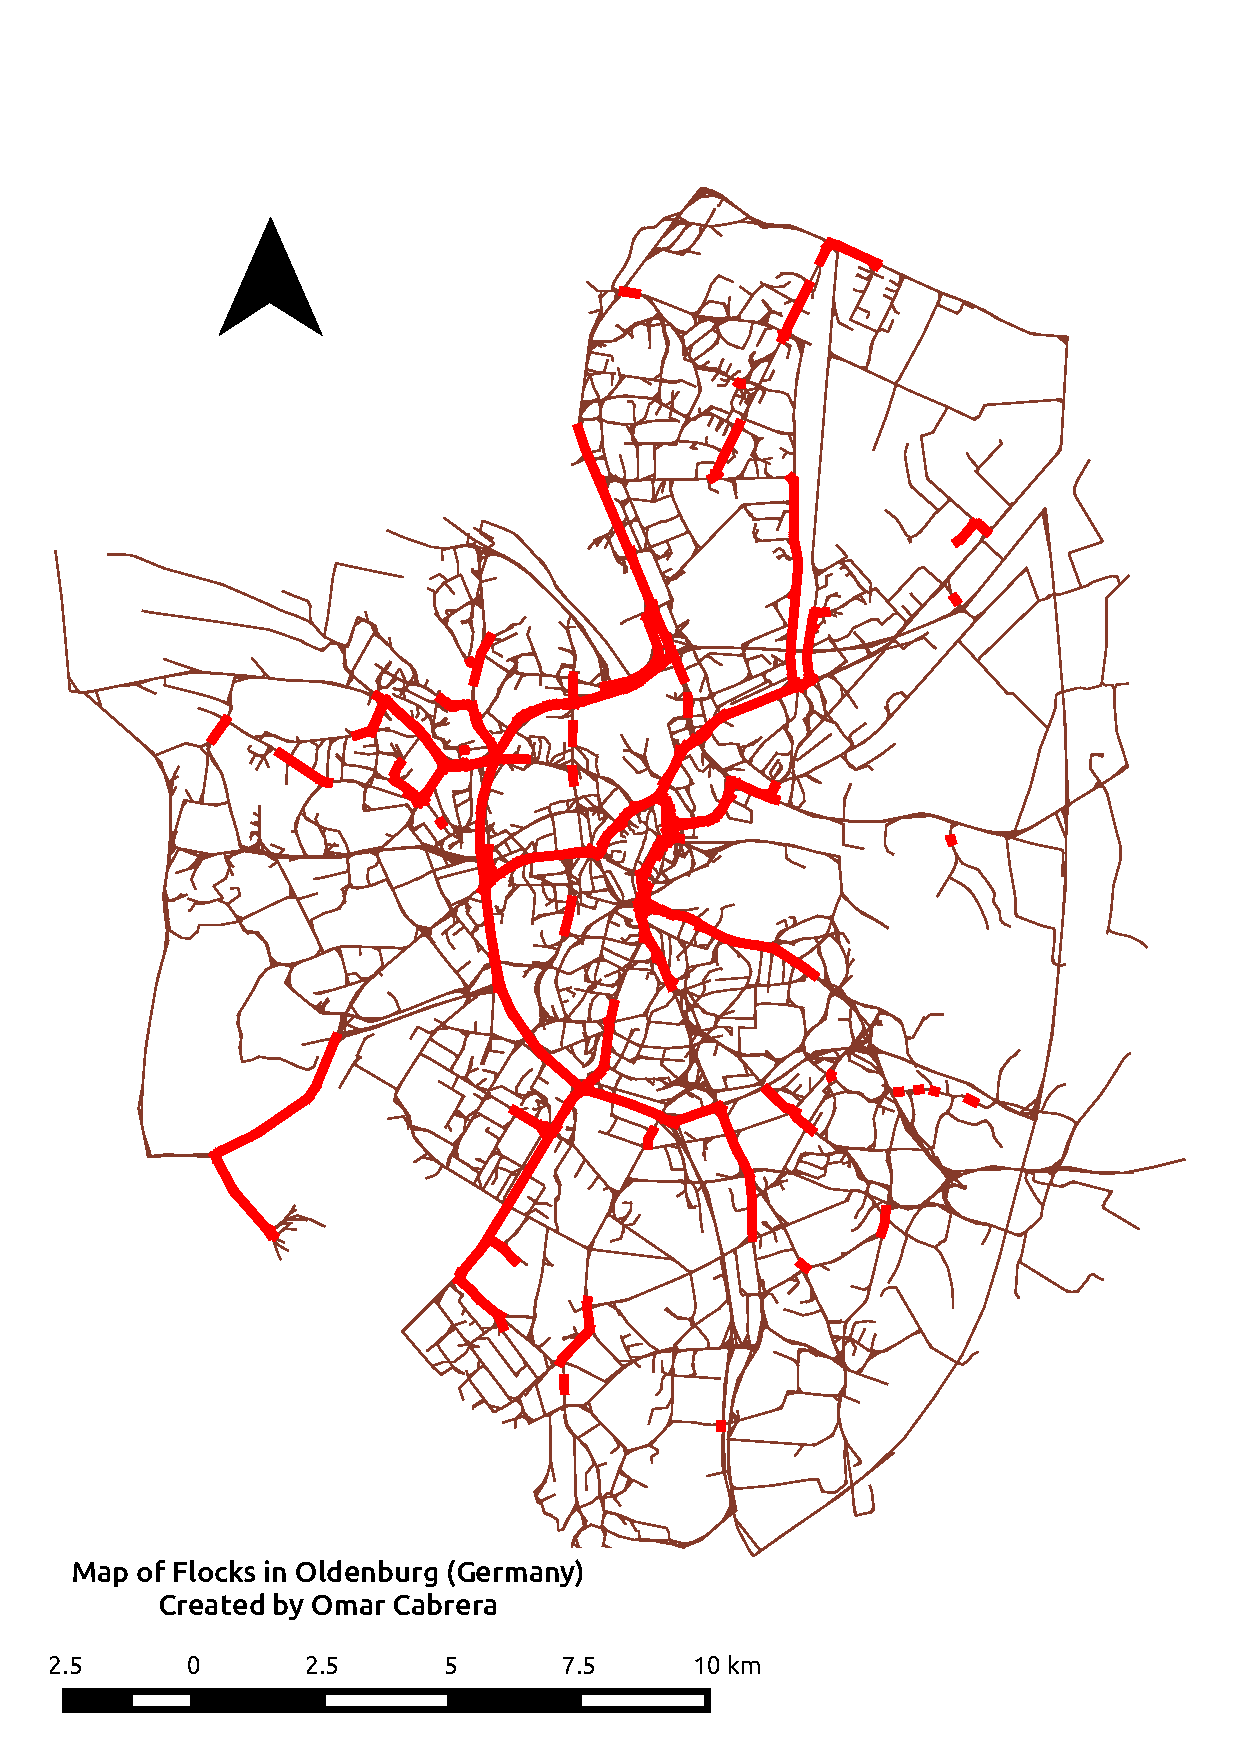
\includegraphics[scale=0.3]{pictures/bfe.pdf}}
  \subfigure[LCMFlock]{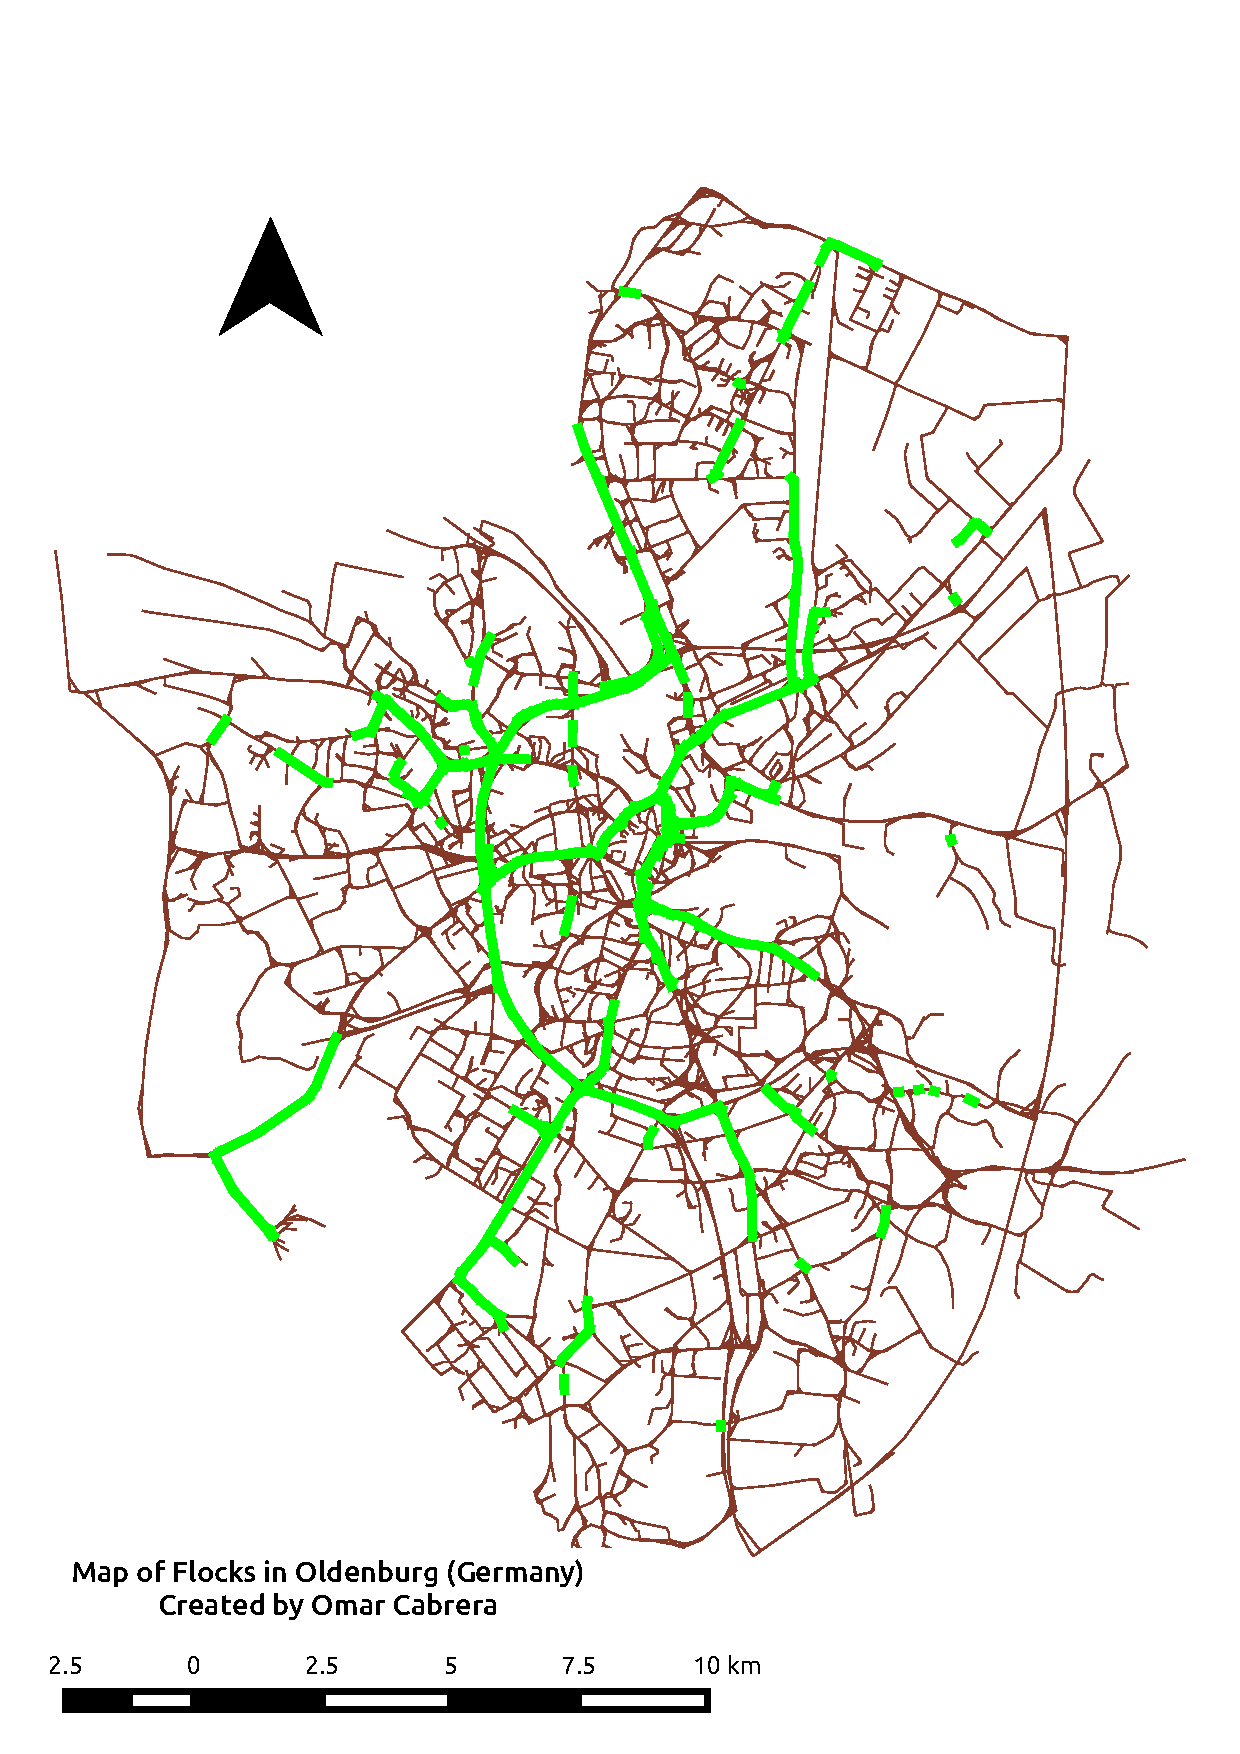
\includegraphics[scale=0.3]{pictures/lcm.pdf}}
  \subfigure[FP-FlockOnline]{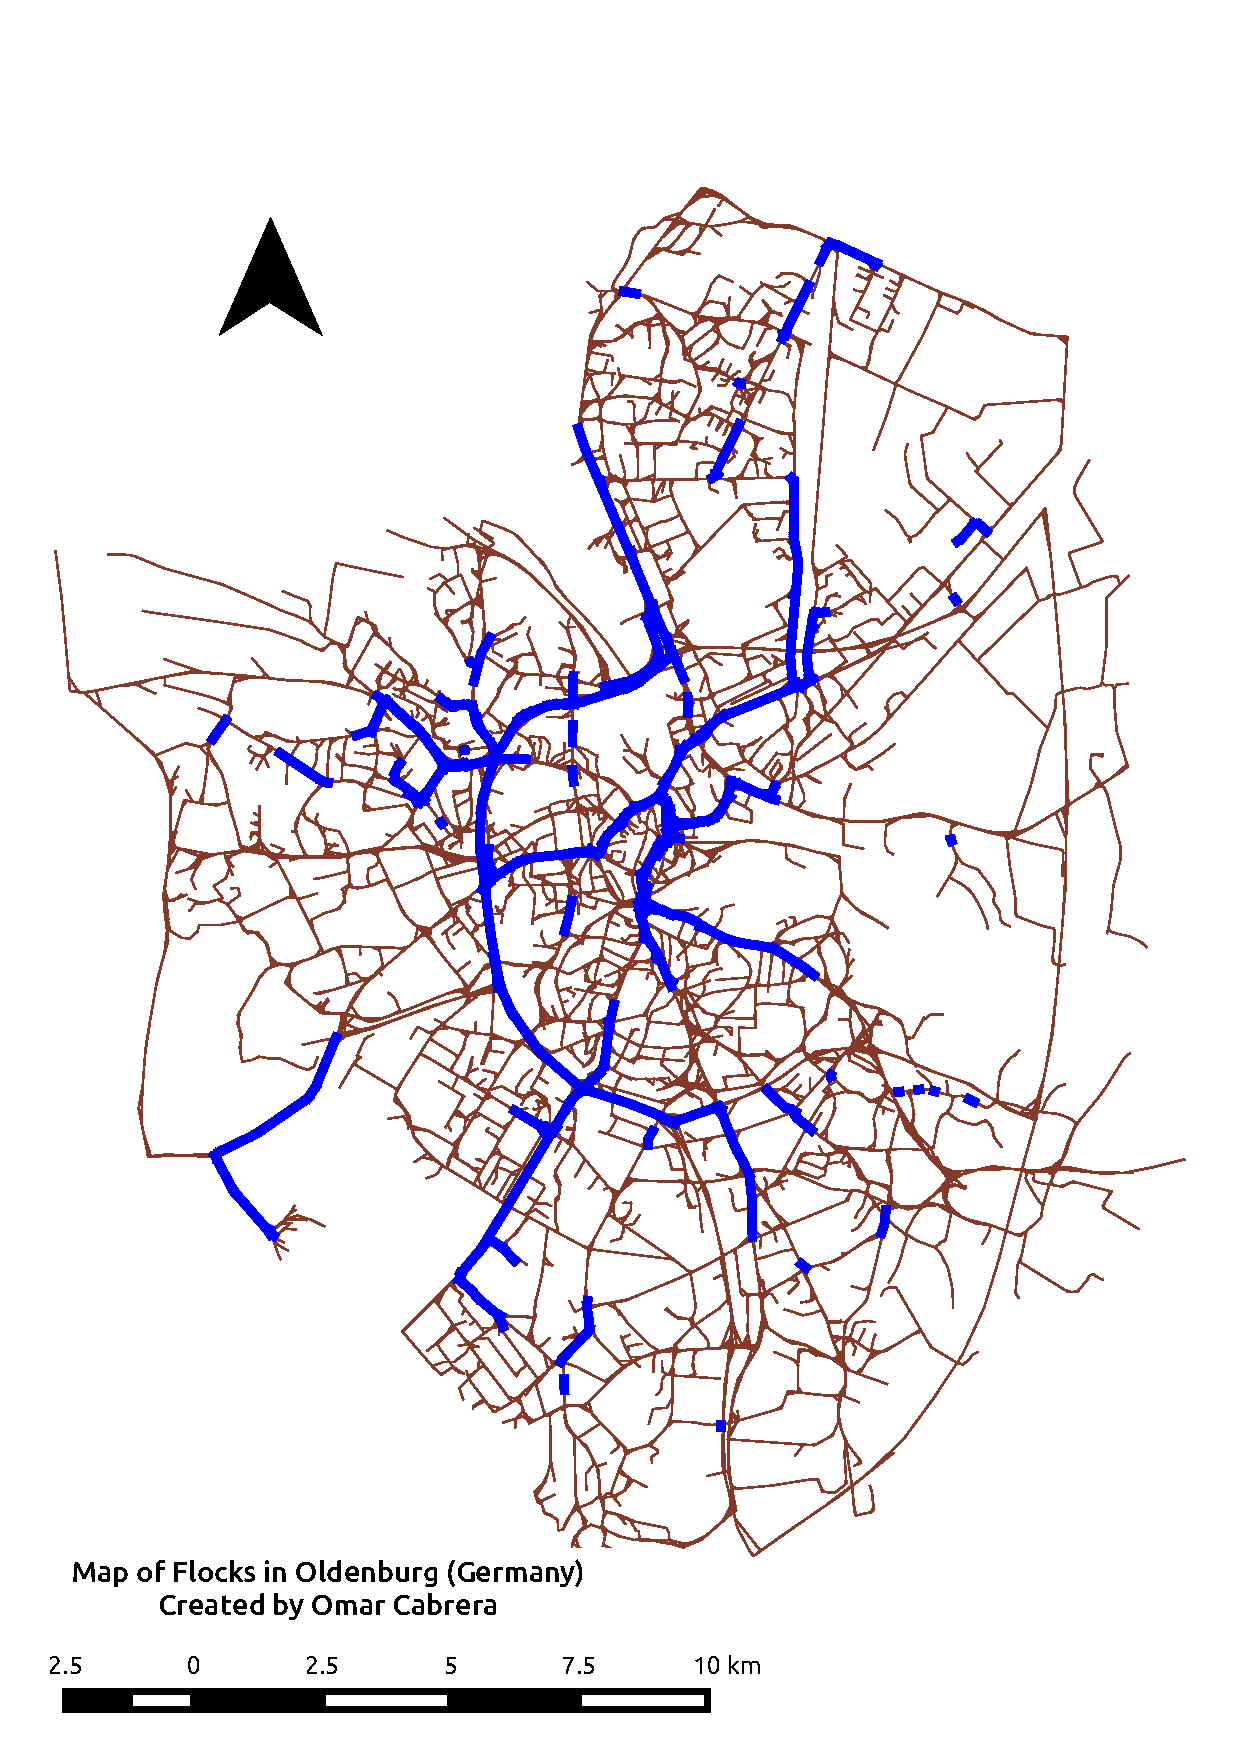
\includegraphics[scale=0.3]{pictures/fpflockOnline.pdf}}
  \subfigure[FP-FlockOffline]{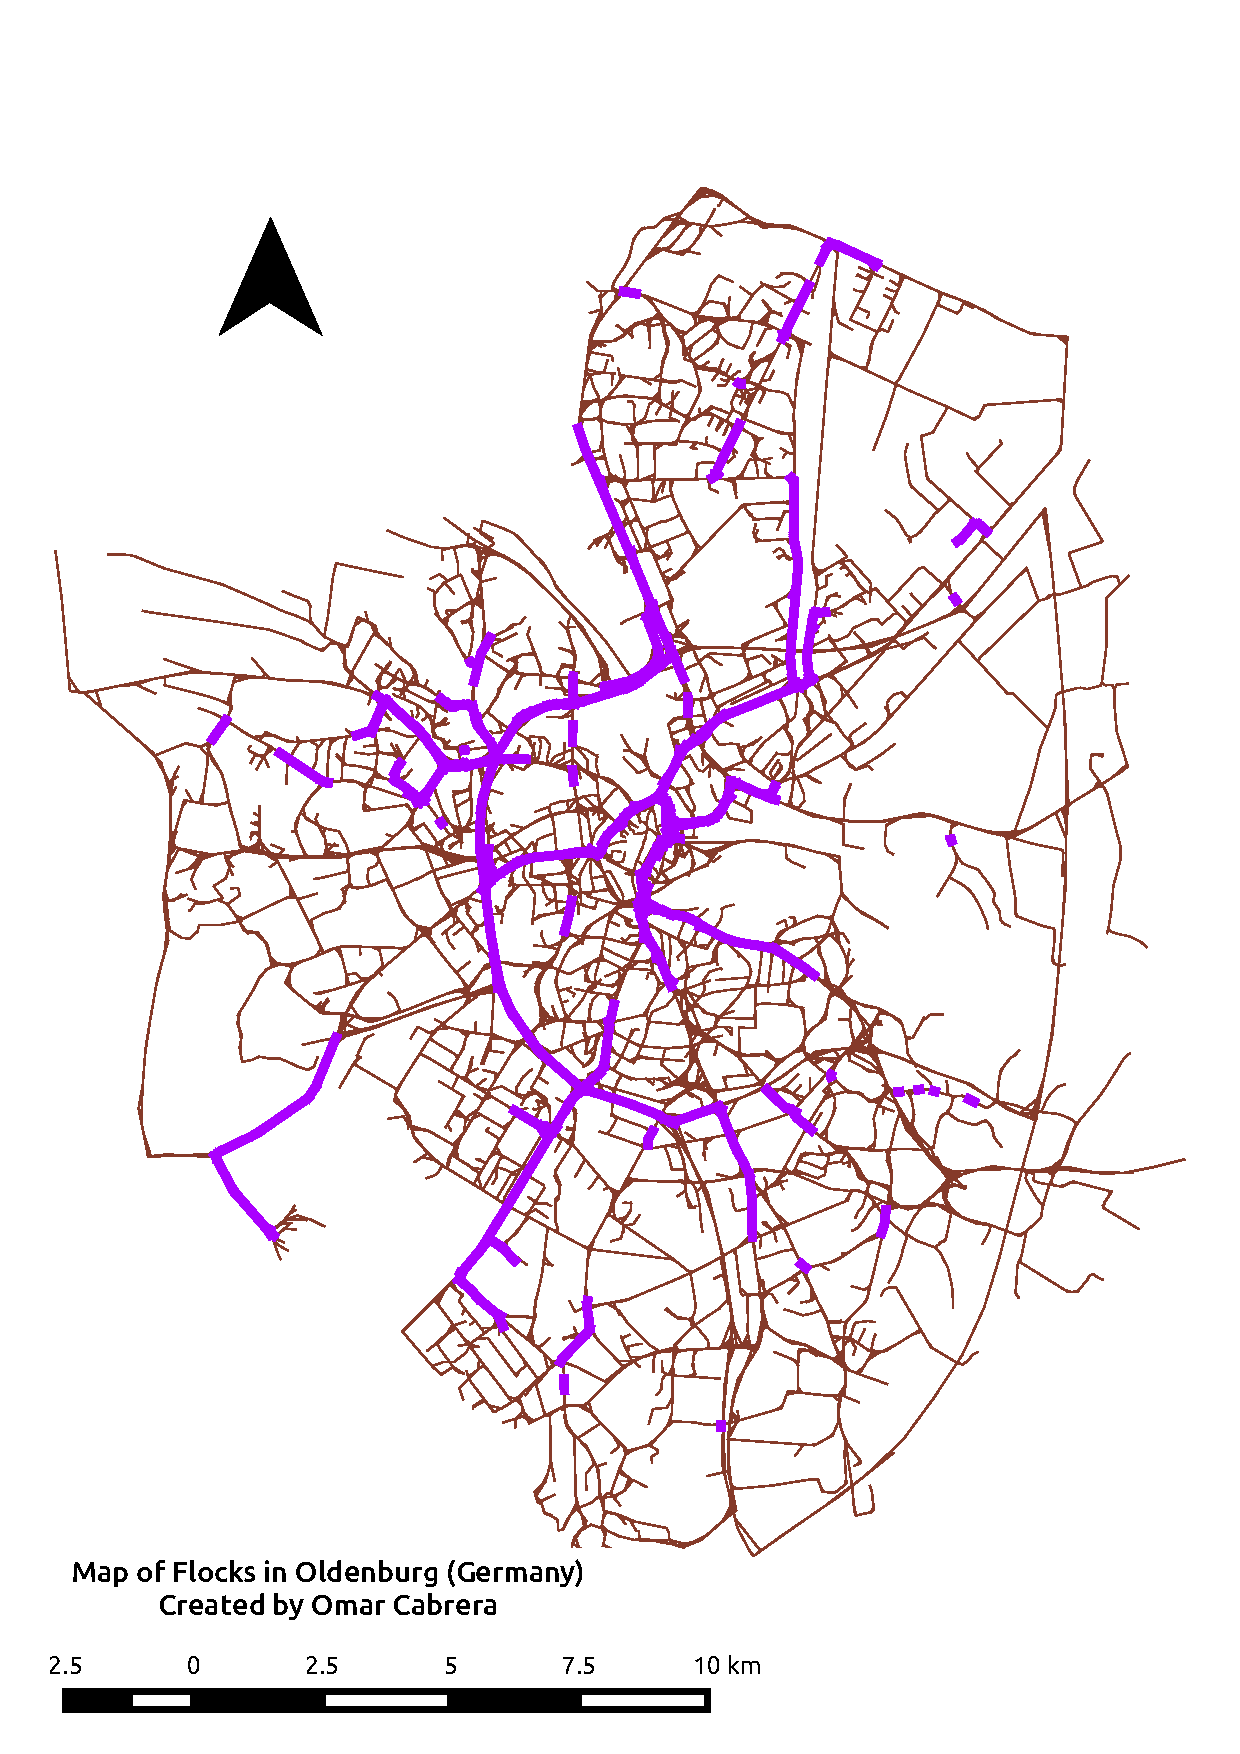
\includegraphics[scale=0.3]{pictures/fpflockOffline.pdf}}
  
  \caption{Visualización Oldenburg}
  \label{fig:validation}
\end{figure}
